\chapter{Grundlagen}

\section{Digitale Plattformen als disruptive Innovation}

\subsection{Definition und begriffliche Abgrenzung}

\newpage

\subsection{Wertschöpfung auf digitalen Plattformen}

\newpage

\subsection{Cloud-Computing auf digitalen Plattformen}

\newpage

\subsection{SAP Business Technology Platform}


\newpage


\section{Die deutsche Versicherungsbranche}

\subsection{Definition und Grundprinzipien der Versicherung}

Aufgrund der kontinuierlichen Weiterentwicklung des Versicherungsmarktes und der wachsenden Teilnahme unterschiedlicher Wirtschaftsdisziplinen an der Versicherungswissenschaft gibt es heutzutage eine Vielzahl von Definition für den Begriff der Versicherung. Wird sich bei dem Begriff auf die ökonomischen Gesichtspunkte konzentriert, wird in der Literatur insbesondere auf den Wirtschaftswissenschaftler Dieter Farny verwiesen, welcher das Versicherungsprodukt, auch Versicherung oder Police genannt, definiert als die: 

\glqq Deckung eines im Einzelnen ungewissen, insgesamt geschätzten Mittelbedarfs auf der Grundlage des Risikoausgleichs im Kollektiv und in der Zeit.\grqq \autocite[S. 8f.]{FARNY2011}

Folglich ist die Versicherung ein Produkt zur Deckung von Sicherheitsbedürfnissen, indem es Risiken auf eine Gefahrengemeinschaft, das Kollektiv überträgt. Die Befriedigung dieser Sicherheitsbedürfnisse umfassen die Absicherung von materiellen als auch beruflichen Risiken und sind auf der zweiten Ebene der Maslowschen Bedürfnispyramide zu finden. \autocite[Vgl.][S. 30]{BECKER2019} Das zugrunde liegende Konzept wird als Risikotransfer bezeichnet, bei dem der Versicherungsnehmer gegen Zahlung einer Prämie das Risiko auf den Versicherer überträgt. Beim Eintreten eines entsprechenden Schadens, dem Versicherungsfall, erhält der Versicherungsnehmer von der Versicherung einen Schadensausgleich. Dieser Risikoausgleichseffekt wird von Versicherungsunternehmen genutzt, um die systematische Übernahme von Risiken mit einem im Hinblick auf die Gewinnmöglichkeiten akzeptablen unternehmerischen Risiko durchzuführen. \autocite[Vgl.][S. 9]{FARNY2011}
Grundvoraussetzung ist hierbei, dass der Umfang der Schäden statistisch abschätzbar und dadurch der benötigte Beitrag jedes Mitglieds des Kollektivs mathematisch bestimmbar ist. Aufgrund dieser Kombinationen von Risikotransfer und Prämienzahlung werden Versicherungsunternehmen(VU) auch als Finanz- und Risikointermediäre bezeichnet. \autocite[Vgl.][S. 53]{ZWACK2017}

Grundsätzlich wird zwischen zwei Arten von Versicherungsunternehmen unterschieden: Erstversicherer und Rückversicherer. Erstere schließen ausschließlich Versicherungsgeschäfte mit gewerblichen Unternehmen, privaten und öffentlichen Haushalten ab, währenddessen Rückversicherer das daraus resultierende Risiko der Erstversicherer übernehmen.\autocite[Vgl.][S. 240f.]{FARNY2011} Im Rahmen dieser Arbeit werden insbesondere Kfz-Versicherer betrachtet, welche der Gruppe der Erstversicherer zuzuordnen sind.

Darüber hinaus sind deutsche Erstversicherer durch verschiedene regulatorische Anforderungen wie dem Versicherungsaufsichtsgesetz (VAG) und der Solvency II-Richtlinie der Europäischen Union verpflichtet, um die Stabilität und Integrität des Versicherungsmarktes zu wahren. \autocite[Vgl.][]{BAFIN2016} Eine der fundamentalen Vorschriften ist die Spartentrennung nach § 6 II VAG. Demnach müssen Erstversicherungsunternehmen getrennte Geschäftsbereiche für Lebens-, Kranken- und Kompositversicherungen führen. Zu Gruppe der Kompositversicherungen, welche auch als Schaden- und Unfallversicherung bezeichnet wird, zählen seit dem 30.06.1990 alle Versicherungen, die nicht zur Lebens- und Krankenversicherung gehören. \autocite[Vgl.][S. 241-243]{FARNY2011} In der Praxis führt das Spartentrennungsprinzip häufig zur Bildung von größeren Mutterkonzernen, bei denen eine Holding über mehrere rechtlich selbstständige Versicherungsunternehmen verfügt. (siehe Abbildung \vref{fig:StVKonzern}). Eine beispielhafte Konzernstruktur der AXA SE ist im Anhang ... zu entnehmen. 

\begin{figure}[h]
    \centering
    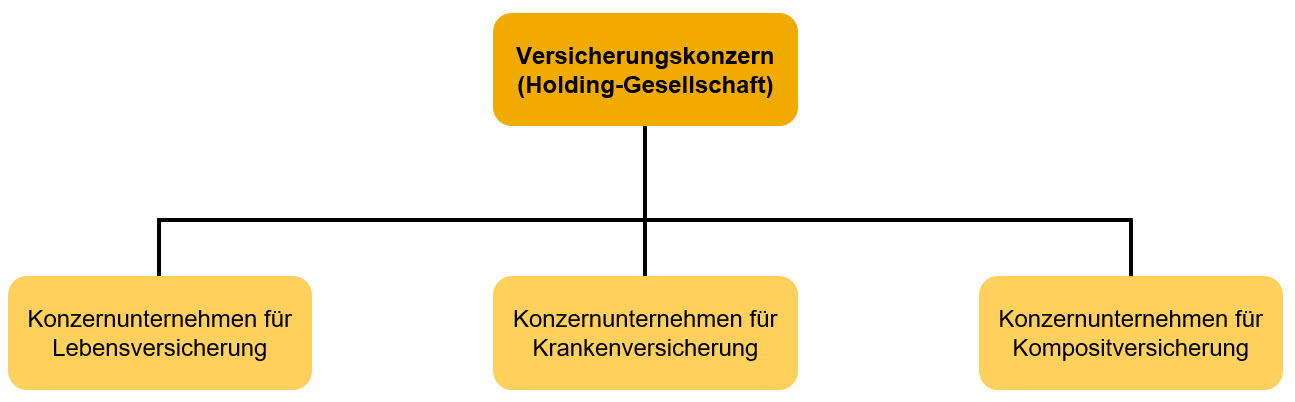
\includegraphics[width=1\textwidth]{img/Struktur_VKonzern2.jpg}
    \caption[Struktur eines Versicherungskonzerns]{Struktur eines Versicherungskonzerns\autocite{StVKonzern}}
    \label{fig:StVKonzern}
\end{figure}
\footnotetext{Vgl. eigene Darstellung angelehnt an: Nguyen, 2013, S.172}

\newpage

\subsection{Aufbau und Besonderheit der Kfz-Versicherungssparte}

Die Kraftfahrtversicherung ist mit einem Volumen von 29 Millionen € in 2021 die größte Sparte in der Schadens- und Unfallversicherung.\autocite[Vgl.][]{GDVSUV} Zu ihr gehören die Kfz-Haftpflichtversicherung, die Fahrzeugversicherung, welche aus der Voll- und Teilkaskoversicherung besteht, sowie die Kraftfahrtunfallversicherung.\autocite[Vgl.][S. 8]{MURINGER2000}

\autocite[Vgl.][]{GDVKFZ}

\begin{figure}[h]
    \centering
    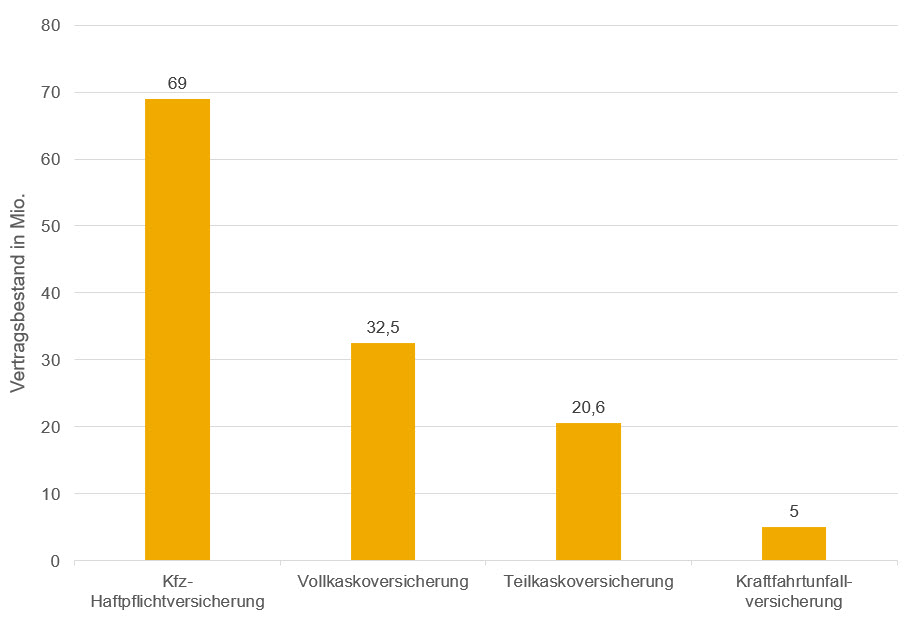
\includegraphics[width=1\textwidth]{img/KfzV_Bestände_an_Verträgen_2021.pdf}
    \caption[Bestände an Verträgen in der Kfz-Versicherung in Deutschland 2021]{Bestände an Verträgen in der Kfz-Versicherung in Deutschland 2021\autocite{KfzVVBestand}}
    \label{fig:KfzVVBestand}
\end{figure}
\footnotetext{Vgl. eigene Darstellung angelehnt an: Nguyen, 2013, S.172}

Wie in Abbildung \vref{fig:KfzVVBestand} zu erkennen, macht die Kfz-Haftpflichtversicherung den größten Teil der Kfz-Versicherung aus. Sie gehört zu den Pflichtversicherungen und deckt den Schaden, der durch die Fahrzeugverwendung gegenüber einem Dritten entsteht, ab. \autocite[Vgl.][S. 81]{STADLER2008}

Die Fahrzeugversicherung, welche umgangssprachlich auch als Kaskoversicherung bezeichnet wird, ist in die Fahrzeugteil- und die Fahrzeugvollversicherung untergliedert. Der wesentliche Unterschied zwischen den beiden Versicherungsarten besteht in dem Leistungsumfang. So sind bei der Fahrzeugteilversicherung ausschließlich, die durch Brand, Diebstahl, Elementarereignisse und Wildschäden verursacht wurden, gedeckt. Bei der Vollversicherung werden darüber hinaus auch Schäden abgedeckt, die durch den Versicherungsnehmer selbst verursacht werden.\autocite[Vgl.][S. 48]{FELTEN2012}

Die Kraftfahrtunfallversicherung oder auch Insassenunfallversicherung genannt, deckt im Falle eines Unfalls Personenschäden von Insassen eines Fahrzeugs ab. Versichert sind alle Unfälle, welche ausschließlich in unmittelbaren Zusammenhang mit dem Gebrauch eines Fahrzeugs entstehen, wie zum Beispiel das Fahren, Ein- und Aussteigen oder das Be- und Entladen.\autocite[Vgl.][S. 6f]{STADLER1998} Dennoch werden aufgrund der großen Deckung der Leistung durch andere Versicherungen, wie in Abbildung … zu erkennen, verhältnismäßig wenige Insassenunfallversicherungen abgeschlossen. So kommt bei einem fremdverschuldeten Unfall die Kfz-Haftpflichtversicherung des Unfallverursachers für alle Unfallopfer auf. Bei selbst verschuldeten Unfällen sind die Mitfahrer durch die Kfz-Haftpflichtversicherung des Fahrers bzw. des Halters abgesichert. Somit ist das Abschließen einer Insassenunfallversicherung vor allem zum Schutz des Fahrers selbst sinnvoll.\autocite[Vgl.][S. 173f]{LAMMERS2006} In der Praxis wird hierfür allerdings häufig auf andere Alternativen wie die private Unfallversicherung zurückgegriffen.\autocite[Vgl.][]{GRATZLA2018}  

Darüber hinaus gibt es in der Kfz-Versicherungssparte einen enormen Konkurrenzdruck. So versuchen die einzelnen Anbieter insbesondere im Herbst neue Kunden zu gewinnen, da die Verträge der Versicherungsnehmer in der Regel zum 31.12 eines jeden Jahres enden und folglich bis zum 30.11 eines jeden Jahres gekündigt werden können.\autocite[Vgl.][]{WARENTEST2022} Des Weiteren veröffentlich der Gesamtverband der deutschen Versicherer jedes Jahr im Herbst ausgehend von der Unfallhäufigkeit der verschiedenen Fahrzeugtypen, die Preiskategorien für die einzelnen Typklassen . Daraufhin passen die meisten Versicherer ihre Beiträge an, was wiederum ihren Kunden ermöglicht, von einem Sonderkündigungsrecht Gebrauch zu machen.\autocite[Vgl.][]{NUS2022} Diese beiden Faktoren führen dazu, dass die Versicherer insbesondere im Herbst versuchen, neue Kunden mit Sonderangeboten und Rabatten für sich zu gewinnen. 

Dabei sind die Kunden oftmals bereits neben der Kfz-Versicherung weitere Policen beim gleichen Anbieter abzuschließen. Um von diesem Interesse und der Wechselbereitschaft der Kunden zu profitieren, sind die Versicherungsunternehmen bereit, kleinere Profite bis hin zu Verlusten bei der Kfz-Versicherung in Kauf zu nehmen.\autocite[Vgl.][]{HARTUNG2019} Dies lässt sich ebenfalls an der Schadensquote der Kfz-Versicherungen erkennen, welche zwischen 2015 und 2021 bei durchschnittlich 96,4 \% lag. Sie stellt das Verhältnis zwischen den Versicherungsleistungen und den Beitragseinnahmen dar.\autocite[Vgl.][]{GDVKFZ}  



\newpage
